\documentclass[fleqn]{article}
\usepackage{xcolor}
\usepackage{amsmath}
\usepackage{graphicx}
\usepackage{wrapfig}
\usepackage[margin=0.5in]{geometry}
\usepackage{caption}
\usepackage[font={color=black!30!white},figurename=Fig.,labelfont={it}]{caption}
\usepackage{tabto}

\title{Week 1 Computer Vision Notes}
\date{3-25-2020}
\author{Maxwell Li}

\begin{document}
  \color{black!30!white}
  \pagecolor{black!80!white}
  \maketitle
  \tableofcontents
  \setcounter{secnumdepth}{0}
  \pagenumbering{arabic}
  \newpage

  \section{\textbf{Section 1: Getting Started with Images}}
    \subsection{Introduction}
    Some things we will learn\\
    \quad - What is color?\\
    \quad - How does a camera see an image?\\
    \quad - How to read/write images?\\
    \quad - How to manipulate pixels?\\
    \quad - Alot more!

    \subsection{How is An Image Formed}
    Throughout history the phenomena of imaging has been explored by many ancient civilizations. The most used primitive form of a camera that has been used was the pinhole camera. The pinhole camera works by taking the light waves that bounce off of an object and projecting them through a small hole.

    \begin{figure}[h]
      \centering
      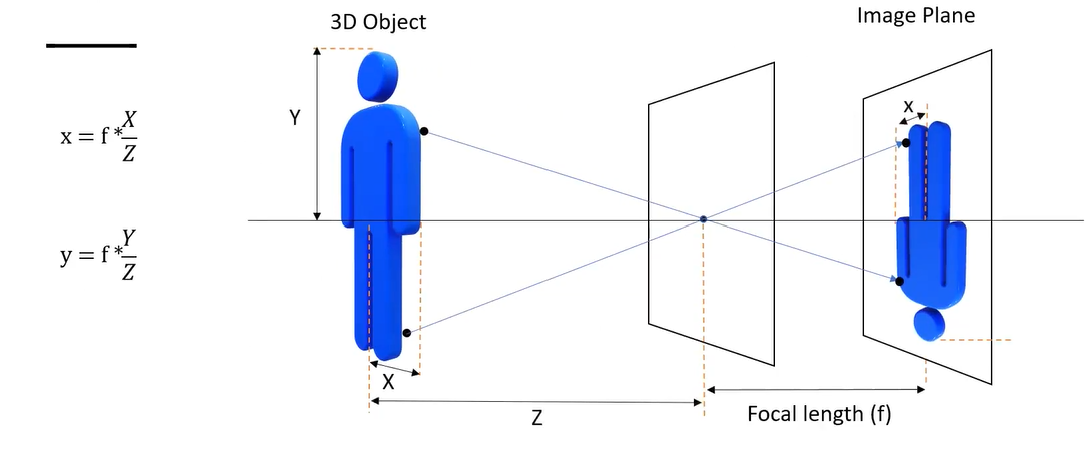
\includegraphics[width = 250pt]{pinholecamera.png}
      \caption{PinHole Camera Example}
      \label{fig: Pinhole Camera}
    \end{figure}

    %

    \subsection{Image Formation}
    Inside of a camera there is a sensor that is a large grid of nodes. These nodes are what eventually become ``pixels'''. Each node on the sensor gets a value between 0 and 255 which represents the digital grayscale image. The value for each node is determined by the strength of the light that hits it. The stronger the light the closer the value is to 255 as 255 is white and 0 is black. Each pixel is essentially an 8 bit representation of the intensity of the light at that position on the sensor.

    \begin{figure}[h!]
      \centering
      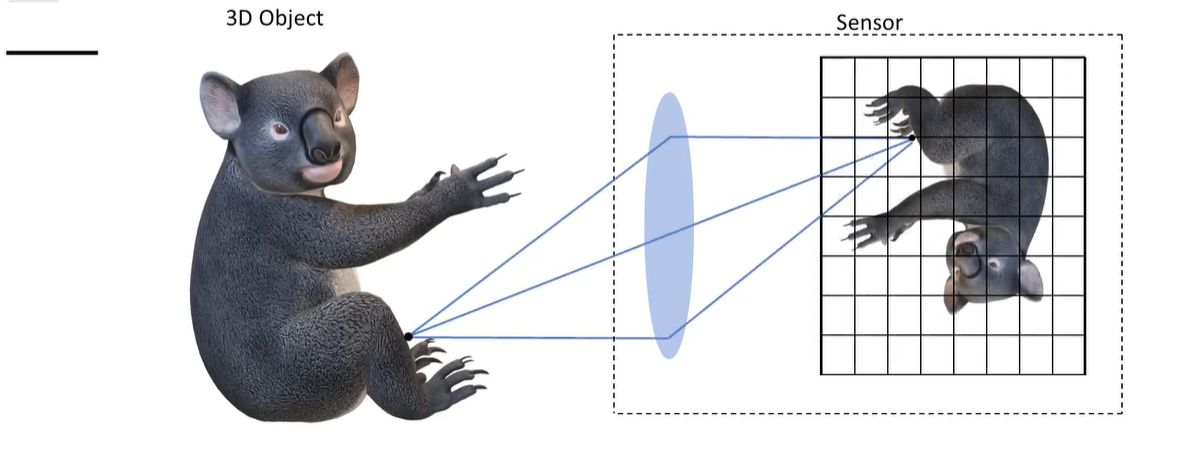
\includegraphics[width=250pt]{koala.png}
      \caption{Greyscale Digitalization }
      \label{fig: Greyscale Representation of an Image}
    \end{figure}



    \newpage
    \clearpage
    \subsection{Bayer Pattern}
    Every pixed only records one color: red, green, or blue. The human eye is much more sensitive to green light than blue or red. The full RGB Image is then formed through a process called demosaicing where 2 two missing values from each pixel are calculated from the neighbouring pixels\\
    \textbf{For example:} If a pixel records the red value, based on the pixels around it the pixel will interpolate what the correct hue for the 2 missing colors.

    \begin{figure}[h!]
      \centering
      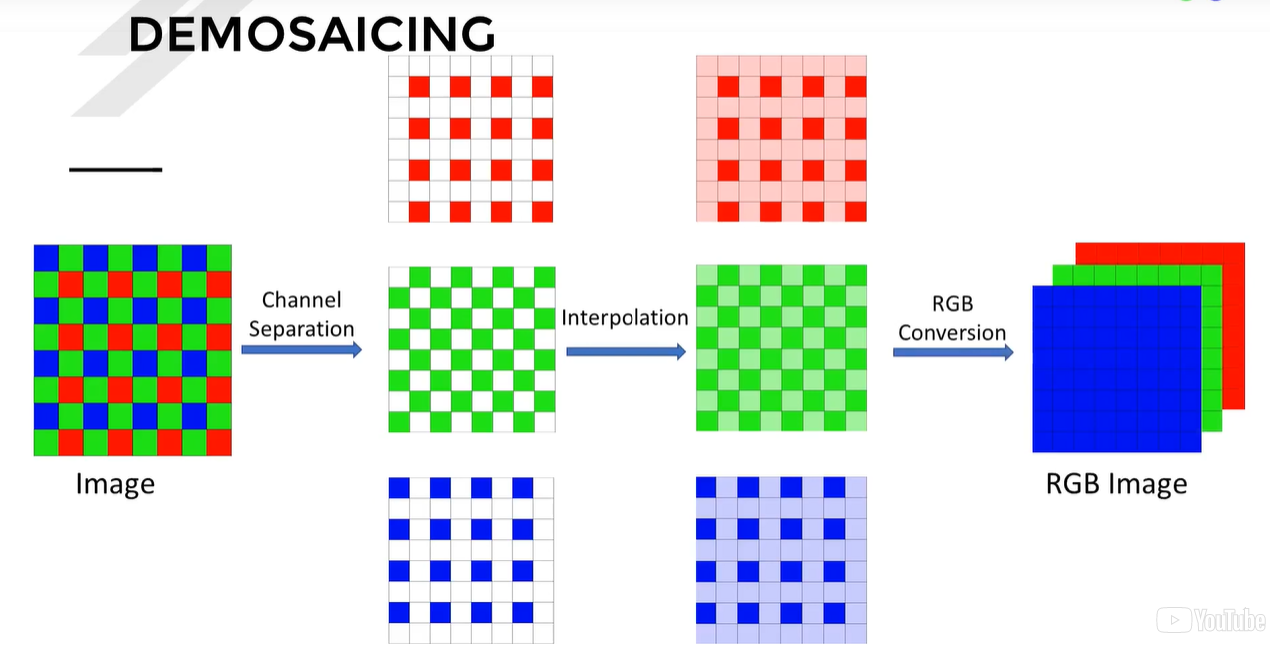
\includegraphics[width=550pt]{demosaicing.png}
      \caption{Process of Demosaicing}
      \label{fig: How the total RGB Image is found through demosaicing}
    \end{figure}

    \subsection{Image Format}
    Once a RGB image is created, they are typically stored and compressed as either Joint Photographic Expert Group (JEPGs) or Portable Network Graphics (PNGs).

    \subsubsection{Image Storage}
    Within a JPEG file the image is broken up into two parts. There is the Image Header and the Data.\\
    \tab - Image Header\\
    \tab\tab - Width\\
    \tab\tab - Height\\
    \tab\tab - No. of channel\\
    \tab\tab - Color Profile\\
    \tab\tab - No. of bits per pixel\\
    The second part is the data which actually contains the RBG values

    \subsection{Image in OpenCV}
    When an image is first read in openCV the image is decompressed and stored in a standardized format. All images are stored into the \textbf{Mat Class} if the C++ version is being used, or a \textbf{Numpy array} if Python is being used.

    \subsubsection{Mat Class}
    The Mat class is similar to a JPEG in structure but the difference is that instead of using RGB values it used BGR. It uses bgr because of historic reasons, aka that is how they initially did it and it makes no sense to back through and change all of the backend code now.








\end{document}
